% !TEX encoding = UTF-8 Unicode
%%%%%%%%%%%%%%%%%%%%%%%%%%%%%%%%%%%%%%%%%
% Beamer Presentation
% LaTeX Template
% Version 1.0 (10/11/12)
%
% This template has been downloaded from:
% http://www.LaTeXTemplates.com
%
% License:
% CC BY-NC-SA 3.0 (http://creativecommons.org/licenses/by-nc-sa/3.0/)
%
%%%%%%%%%%%%%%%%%%%%%%%%%%%%%%%%%%%%%%%%%

%----------------------------------------------------------------------------------------
%	PACKAGES AND THEMES
%----------------------------------------------------------------------------------------

\documentclass{beamer}

\mode<presentation> {

% The Beamer class comes with a number of default slide themes
% which change the colors and layouts of slides. Below this is a list
% of all the themes, uncomment each in turn to see what they look like.

%\usetheme{default}
%\usetheme{AnnArbor}
%\usetheme{Antibes}
%\usetheme{Bergen}
%\usetheme{Berkeley}
%\usetheme{Berlin}
%\usetheme{Boadilla}
%\usetheme{CambridgeUS}
%\usetheme{Copenhagen}
%\usetheme{Darmstadt}
%\usetheme{Dresden}
%\usetheme{Frankfurt}
%\usetheme{Goettingen}
%\usetheme{Hannover}
%\usetheme{Ilmenau}
%\usetheme{JuanLesPins}
%\usetheme{Luebeck}
\usetheme{Madrid}
%\usetheme{Malmoe}
%\usetheme{Marburg}
%\usetheme{Montpellier}
%\usetheme{PaloAlto}
%\usetheme{Pittsburgh}
%\usetheme{Rochester}
%\usetheme{Singapore}
%\usetheme{Szeged}
%\usetheme{Warsaw}

% As well as themes, the Beamer class has a number of color themes
% for any slide theme. Uncomment each of these in turn to see how it
% changes the colors of your current slide theme.

%\usecolortheme{albatross}
%\usecolortheme{beaver}
%\usecolortheme{beetle}
%\usecolortheme{crane}
%\usecolortheme{dolphin}
%\usecolortheme{dove}
%\usecolortheme{fly}
%\usecolortheme{lily}
%\usecolortheme{orchid}
%\usecolortheme{rose}
%\usecolortheme{seagull}
%\usecolortheme{seahorse}
%\usecolortheme{whale}
%\usecolortheme{wolverine}

%\setbeamertemplate{footline} % To remove the footer line in all slides uncomment this line
%\setbeamertemplate{footline}[page number] % To replace the footer line in all slides with a simple slide count uncomment this line

%\setbeamertemplate{navigation symbols}{} % To remove the navigation symbols from the bottom of all slides uncomment this line
}

\usepackage{graphicx} % Allows including images
\usepackage{booktabs} % Allows the use of \toprule, \midrule and \bottomrule in tables
\usepackage{xeCJK}
\usepackage{color}
\usepackage{listings}
\usepackage{tikz}


%----------------------------------------------------------------------------------------
%	TITLE PAGE
%----------------------------------------------------------------------------------------

\title[File]{File} % The short title appears at the bottom of every slide, the full title is only on the title page

\author{张海宁} % Your name
\institute[贵大计算机] % Your institution as it will appear on the bottom of every slide, may be shorthand to save space
{
贵州大学 \\ % Your institution for the title page
\medskip
\textit{hnzhang1@gzu.edu.cn} % Your email address
}
\date{\today} % Date, can be changed to a custom date

\begin{document}

\begin{frame}
\titlepage % Print the title page as the first slide
\end{frame}

\begin{frame}
\frametitle{Overview} % Table of contents slide, comment this block out to remove it
\tableofcontents % Throughout your presentation, if you choose to use \section{} and \subsection{} commands, these will automatically be printed on this slide as an overview of your presentation
\end{frame}

%----------------------------------------------------------------------------------------
%	PRESENTATION SLIDES
%----------------------------------------------------------------------------------------

%------------------------------------------------
\section{文件结构} % Sections can be created in order to organize your presentation into discrete blocks, all sections and subsections are automatically printed in the table of contents as an overview of the talk
%------------------------------------------------
\begin{frame}
\frametitle{文件结构}
Linux中,一切(或几乎一切)都是文件。

这意味着针对串口,打印机等设备的操作可以像文件一样来进行操作。

文件可以分为以下两类:
\begin{enumerate}
\item
目录

特殊的文件
\item
文件和设备
\end{enumerate}
Linux系统是通过inode来识别文件的,文件名只是为了用户的使用方便。
\end{frame}
\begin{frame}
\frametitle{inode}
inode是linux系统中的一种数据结构。它存储了文件系统对象(包括文件、目录、设备文件、socket、管道, 等等)的元信息数据,但不包括数据内容或者文件名。


文件系统中每个“文件系统对象”对应一个“inode”数据,并用一个整数值来辨识。这个整数常被称为inode号码(“i-number”或“inode number”)。

Inode存储了文件系统对象的一些元信息,如所有者、访问权限(读、写、执行)、类型(是文件还是目录)、内容修改时间、inode修改时间、上次访问时间、对应的文件系统存储块的地址,等等。

\textcolor{red}{一个文件系统对象可以有多个别名,但只能有一个inode},并用这个inode来索引文件系统对象的存储位置。

使用stat系统调用可以查询一个文件的inode号码及一些元信息。
\end{frame}
%\subsection{System Calls} % A subsection can be created just before a set of slides with a common theme to further break down your presentation into chunks

\begin{frame}
\frametitle{目录}
\begin{tikzpicture}
\node(/) at (7,10) {/};
\node(bin) at (5,8) {bin};
\node(home) at (7,8) {home};
\node(dev) at (9,8) {dev};
\draw (bin) -- (/) -- (dev);
\draw (/) -- (home);
\node (zhn) at (5,6) {zhn};
\node (wys) at (7,6) {wys};
\node (students) at (9,6) {students};
\draw (home) -- (zhn);  
\draw (home) -- (wys); 
\draw (home) -- (students); 
%\node (public\_html) at (3,4) {public\_html};
\node (linux) at (2,4) {linux};
\node (javaweb) at (7,4) {javaweb};
%\draw (zhn) -- (public\_html);
\draw (zhn) -- (linux);
\draw (zhn) -- (javaweb);


\end{tikzpicture}
\end{frame}
\begin{frame}
\frametitle{文件和设备}
硬件设备在Linux系统中也通常被映射为文件,比如U盘,会被Linux系统自动挂载到一个目录下面。

Linux系统中,比较重要的设备文件有:
\begin{itemize}
\item
/dev/console

这个设备代表系统控制台,通常是指“活跃的虚拟控制台”,或者是一个特殊的控制台窗口。
\item
/dev/tty

如果一个进程有控制终端的话,那么,特殊文件/dev/tty就是这个控制终端的别名。
\item
/dev/null

这是空设备,任何写向这个设备(文件)的输出都将被丢弃。
\end{itemize}
\end{frame}


%------------------------------------------------
\section{底层文件访问}
\begin{frame}
\frametitle{与底层文件访问有关的几个重要的系统调用}
每个运行中的程序被称为进程,它有一些与之相关的文件描述符,可以通过这些文件描述符来访问打开的文件或设备。在运行程序时,一般有很3个已经打开的文件描述符:0,1,2.(各是什么意思?)

下面列出几个常用的与文件访问有关的系统调用:
\begin{enumerate}
\item
write
\item
read
\item
open
\item
close
\item
ioctl

\end{enumerate}


\end{frame}
\begin{frame}[fragile]
\frametitle{write}
系统调用write的作用是把缓冲区buf的前nbyte写入与文件描述符相关联的文件中去,会返回实际写入的字节数,若未写入任何数据则返回0,返回-1表示出现了错误,对应的错误代码会保存在全局变量errno中。
\begin{example}[write系统调用的原型]
\begin{verbatim}
#include <unistd.h>
size_t write(int fildes, const void *buf, size_t nbytes);
\end{verbatim}
\end{example}

\end{frame}



\begin{frame}[fragile]
\frametitle{write}
\begin{example}[write系统调用的使用实例]
\begin{verbatim}
     1  #include<unistd.h>
     2  #include<stdlib.h>
     3  #include<stdio.h>
     4
     5  int main(){
     6    if((write(1,"Here is some data.\n",18)!=18)){
     7      write(2,"A write error has occurred!\n",46);
     8    }
     9   printf("continue?");
    10  exit(0);
    11 }
\end{verbatim}
\end{example}

\end{frame}

\begin{frame}[fragile]
\frametitle{read}
系统调用read的作用是从与文件描述符相关联的文件中读出前nbyte写入到缓冲区buf里,会返回实际读出的字节数,若返回0则表示读到了文件的末尾,返回-1表示出现了错误。
\begin{example}[read系统调用的原型]
\begin{verbatim}
#include <unistd.h>
size_t read(int fildes, void *buf, size_t nbytes);
\end{verbatim}
\end{example}

\end{frame}



\begin{frame}[fragile]
\frametitle{read}
\begin{example}[read系统调用的使用实例]
\begin{verbatim}
     1  #include<unistd.h>
     2  #include<stdlib.h>
     3
     4  int main(){
     5  char buffer[128];
     6  int nread;
     7 nread = read(0,buffer,128);
     8  if(nread==-1){
     9   write(2,"A read error has occurred.\n",27);
    10  }
    11  if((write(1,buffer,nread))!=nread){
    12    write(2,"A write error has occurred.\n",27);
    13  }
    14  exit(0);
    15  }
\end{verbatim}
\end{example}

\end{frame}


\begin{frame}[fragile]
\frametitle{运行read程序的方法}
\begin{columns}
\column{.45\textwidth}
\begin{enumerate}
\item
使用管道输入
\item
使用输入重定向进行输入
\item
直接运行程序,从终端输入
\end{enumerate}
\column{.5\textwidth}
\begin{lstlisting}
cat simple_read.c | ./read
./read < simple_read.c
./read
\end{lstlisting}
\end{columns}
\end{frame}

\begin{frame}[fragile]
\frametitle{open}
系统调用open的作用是\textcolor{red}{创建文件描述符}。这个文件描述符可以提供给read或write系统调用使用。

两个程序打开\textcolor{red}{同一个文件}会得到\textcolor{red}{两个不同的文件描述符},后写入的内容会\textcolor{red}{覆盖}之前写入的内容!
\begin{example}[open系统调用的原型]
\begin{verbatim}
#include <fcntl.h>
#include <sys/types.h>
#include <sys/stat.h>

int open(const char *path, int oflags);
int open(const char *path, int oflags, mode_t mode);
\end{verbatim}
\end{example}

\end{frame}

\begin{frame}
\frametitle{oflags}
oflags是用来指定打开文件方式的参数。open调用必须指定表\ref{主要文件访问模式}中所示的文件访问模式之一。
\begin{table}
\begin{tabular}{cc}
\toprule
\textbf{模式} & \textbf{说明} \\
\midrule
O\_RDONLY & 以只读方式打开\\
O\_WRONLY & 以只写方式打开\\
O\_RDWR & 以读写方式打开\\
\bottomrule
\end{tabular}
\caption{主要文件访问模式}
\label{主要文件访问模式}
\end{table}
\end{frame}
\begin{frame}[fragile]
\frametitle{oflags-II}
oflags参数还可以包含以下可选模式的组合(按位或)。
\begin{table}
\begin{tabular}{cc}
\toprule
\textbf{模式} & \textbf{说明} \\
\midrule
O\_APPEND & 追加数据在文件末尾\\
O\_TRUNC & 丢弃文件原有内容\\
O\_CREAT & 如果需要,就按照mode中给出的访问模式创建文件\\
\bottomrule
\end{tabular}
\caption{可选文件访问模式}
\label{可选文件访问模式}
\end{table}
\textcolor{red}{按位或}
\begin{lstlisting}
/usr/include/sys/fcntl.h
#define O_CREAT  0x0200  /* create if nonexistant */
#define O_TRUNC 0x0400  /* truncate to zero length */
#define O_EXCL  0x0800  /* error if already exists */
\end{lstlisting}
\end{frame}

\begin{frame}[fragile]
\frametitle{O\_CREAT}
当使用带有O\_CREAT标志的open来创建文件时,必须使用带有三个参数格式的open调用。第三个参数mode是几个标志按位或得到的。
\begin{lstlisting}
cat /usr/include/sys/_types/_s_ifmt.h
#define S_IRWXU  0000700  /* [XSI] RWX mask for owner */
#define S_IRUSR  0000400  /* [XSI] R for owner */
#define S_IWUSR  0000200  /* [XSI] W for owner */
#define S_IXUSR  0000100  /* [XSI] X for owner */
#define S_IRWXG  0000070  /* [XSI] RWX mask for group */
#define S_IRGRP  0000040  /* [XSI] R for group */
#define S_IWGRP  0000020  /* [XSI] W for group */
#define S_IXGRP  0000010  /* [XSI] X for group */
#define S_IRWXO  0000007  /* [XSI] RWX mask for other */
#define S_IROTH  0000004  /* [XSI] R for other */
#define S_IWOTH  0000002  /* [XSI] W for other */
#define S_IXOTH  0000001  /* [XSI] X for other */
\end{lstlisting}
\end{frame}

\begin{frame}[fragile]
\frametitle{open}
\begin{example}[open系统调用的使用实例]
\begin{verbatim}
     1 #include <fcntl.h>
     2 #include <sys/types.h>
     3 #include <sys/stat.h>
     4 #include <stdlib.h>
     5
     6 int main(){
     7 open("myfile",O_CREAT,S_IRUSR|S_IWUSR);
     8 exit(0);
     9 }
\end{verbatim}
\end{example}

\begin{lstlisting}
ls -al myfile 
-rw-------  1 hnz  staff  0 Apr 10 00:34 myfile
\end{lstlisting}
\end{frame}
\begin{frame}[fragile]
\frametitle{umask}
文件被创建时,会指定访问权限,比如open使用带有O\_CREAT标志的参数来创建文件时,会指定权限。但最终的文件权限还是要结合umask(\textcolor{red}{也叫用户掩码},是8进制数)码来确定。

\textcolor{red}{open的权限位会与umask的反码做AND操作}。
\begin{lstlisting}
$ umask         # display current value (as octal)
0022
$ umask -S      # display current value symbolically
u=rwx,g=rx,o=rx
\end{lstlisting}
\end{frame}
\begin{frame}
\frametitle{umask值的说明}
\begin{table}
\begin{tabular}{ll}
\toprule
\textbf{umask } & \textbf{Permissions}\\
\midrule
0 & any permission may be set (read, write, execute)\\
1 & setting of execute permission is prohibited (read and write)\\
2 & setting of write permission is prohibited (read and execute)\\
3 & setting of write and execute permission is prohibited (read only)\\
4 & setting of read permission is prohibited (write and execute)\\
5 & setting of read and execute permission is prohibited (write only)\\
6 & setting of read and write permission is prohibited (execute only)\\
7 & all permissions are prohibited from being set (no permissions)\\
\bottomrule
\end{tabular}
\caption{umask值说明}
\end{table}
\end{frame}
\begin{frame}
\frametitle{umask}
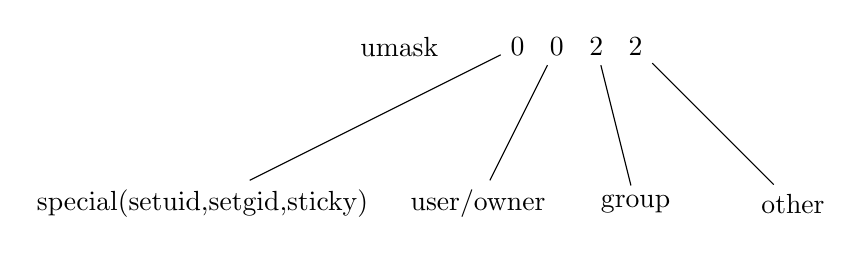
\begin{tikzpicture}
\node () at (3,10) {umask};
\node (U1) at (4.5,10) {0};
\node (U2) at (5,10) {0};
\node (U3) at (5.5,10) {2};
\node (U4) at (6,10) {2};
\node (S) at (0.5,8) {special(setuid,setgid,sticky)};
\node (Usr) at (4,8) {user/owner};
\node (G) at (6,8) {group};
\node (O) at (8,8) {other};
\draw (U1) -- (S);
\draw (U2) -- (Usr);
\draw (U3) -- (G);
\draw (U4) -- (O);
\end{tikzpicture}
\end{frame}
\begin{frame}
\frametitle{special bit in umask}
\textcolor{red}{setuid and setgid} (short for "set user ID upon execution" and "set group ID upon execution", respectively) are Unix access rights flags that allow users to /textcolor{red}{run an executable with the permissions of the executable's owner or group respectively} and to change behaviour in directories. They are often used to allow users on a computer system to run programs with temporarily elevated privileges in order to \textcolor{red}{perform a specific task}. While the assumed user id or group id privileges provided are not always elevated, at a minimum they are specific.

When \textcolor{red}{a directory's sticky bit} is set, the filesystem treats the files in such directories in a special way so \textcolor{red}{only the file's owner, the directory's owner, or root user can rename or delete the file}. Without the sticky bit set, any user with write and execute permissions for the directory can rename or delete contained files, regardless of the file's owner. Typically this is set on the /tmp directory to prevent ordinary users from deleting or moving other users' files.
\end{frame}
\begin{frame}[fragile]
\frametitle{close系统调用}
close系统调用是用来终止一个文件描述符与其对应文件之间关联的,这个文件描述符会被释放并能被重新使用。其返回值为0或-1 。
\begin{example}[close系统调用的原型]
\begin{verbatim}
#include <unistd.h>
int close(int fildes);
\end{verbatim}
\end{example}


\end{frame}
\begin{frame}
\frametitle{实验:拷贝文件}
使用open,read,write这三个系统调用,编写一个程序simple\_copy.c,将一个文件逐个字符(\textcolor{red}{或多个字符})地拷贝到另外一个文件中去。
\end{frame}
\begin{frame}[fragile]
\frametitle{实验:拷贝文件代码}
\begin{lstlisting}
     1 #include <unistd.h>
     2 #include <sys/stat.h>
     3 #include <fcntl.h>
     4 #include <stdlib.h>
     5 int main(){
     6 char c;
     7 int in,out;
     8 in = open("simple_read.c",O_RDONLY);
     9 out = open("copy_example",
              O_WRONLY|O_CREAT,S_IRWXU);
    10 while(read(in,&c,1) ==1 ){
    11 write(out,&c,1);
    12 write(1,&c,1);}
    13 close(in); close(out);
    14 exit(0);
    15 }
\end{lstlisting}
\end{frame}

%-------------------------------------------------
\section{标准I/O库}
\begin{frame}
\frametitle{标准I/O库}
标准I/O库及其头文件stdio.h为底层I/O系统调用提供了一个通用的接口。标准I/O库提供了许多复杂的函数,用于格式化输出和扫描输入,并且具有缓冲功能。

标准I/O库与底层文件描述符很类似,在启到一个程序时,也是有三个流是自动打开的,分别是stdin,stdout,stderr与0,1,2对应。

标准I/O库中的常用文件操作库函数:
\begin{enumerate}
\item
fopen	fclose
\item
fread		fwrite
\item
fflush
\item
fgetc		getc		getchar
\item
fputc		putc		putchar
\item
fgets		gets
\item
printf		fprintf	sprintf
\item
scanf	fscanf	sscanf
\end{enumerate}

\end{frame}
\begin{frame}[fragile]
\frametitle{fopen}
fopen函数类似系统调用read的作用是从与文件描述符相关联的文件中读出前nbyte写入到缓冲区buf里,会返回实际读出的字节数,若返回0则表示读到了文件的末尾,返回-1表示出现了错误。
\begin{example}[read系统调用的原型]
\begin{verbatim}
#include <unistd.h>
size_t read(int fildes, void *buf, size_t nbytes);
\end{verbatim}
\end{example}

\end{frame}
\begin{frame}[fragile]
\frametitle{fread}
系统调用read的作用是从与文件描述符相关联的文件中读出前nbyte写入到缓冲区buf里,会返回实际读出的字节数,若返回0则表示读到了文件的末尾,返回-1表示出现了错误。
\begin{example}[read系统调用的原型]
\begin{verbatim}
#include <unistd.h>
size_t read(int fildes, void *buf, size_t nbytes);
\end{verbatim}
\end{example}

\end{frame}

\begin{frame}[fragile]
\frametitle{fwrite}
系统调用read的作用是从与文件描述符相关联的文件中读出前nbyte写入到缓冲区buf里,会返回实际读出的字节数,若返回0则表示读到了文件的末尾,返回-1表示出现了错误。
\begin{example}[read系统调用的原型]
\begin{verbatim}
#include <unistd.h>
size_t read(int fildes, void *buf, size_t nbytes);
\end{verbatim}
\end{example}

\end{frame}
\begin{frame}[fragile]
\frametitle{fclose}
系统调用read的作用是从与文件描述符相关联的文件中读出前nbyte写入到缓冲区buf里,会返回实际读出的字节数,若返回0则表示读到了文件的末尾,返回-1表示出现了错误。
\begin{example}[read系统调用的原型]
\begin{verbatim}
#include <unistd.h>
size_t read(int fildes, void *buf, size_t nbytes);
\end{verbatim}
\end{example}

\end{frame}
\begin{frame}[fragile]
\frametitle{fflush}
系统调用read的作用是从与文件描述符相关联的文件中读出前nbyte写入到缓冲区buf里,会返回实际读出的字节数,若返回0则表示读到了文件的末尾,返回-1表示出现了错误。
\begin{example}[read系统调用的原型]
\begin{verbatim}
#include <unistd.h>
size_t read(int fildes, void *buf, size_t nbytes);
\end{verbatim}
\end{example}

\end{frame}

\begin{frame}[fragile]
\frametitle{fseek}
系统调用read的作用是从与文件描述符相关联的文件中读出前nbyte写入到缓冲区buf里,会返回实际读出的字节数,若返回0则表示读到了文件的末尾,返回-1表示出现了错误。
\begin{example}[read系统调用的原型]
\begin{verbatim}
#include <unistd.h>
size_t read(int fildes, void *buf, size_t nbytes);
\end{verbatim}
\end{example}

\end{frame}
\begin{frame}[fragile]
\frametitle{fgetc,getc,getchar}
系统调用read的作用是从与文件描述符相关联的文件中读出前nbyte写入到缓冲区buf里,会返回实际读出的字节数,若返回0则表示读到了文件的末尾,返回-1表示出现了错误。
\begin{example}[read系统调用的原型]
\begin{verbatim}
#include <unistd.h>
size_t read(int fildes, void *buf, size_t nbytes);
\end{verbatim}
\end{example}

\end{frame}
\begin{frame}[fragile]
\frametitle{fputc,putc,putchar}
系统调用read的作用是从与文件描述符相关联的文件中读出前nbyte写入到缓冲区buf里,会返回实际读出的字节数,若返回0则表示读到了文件的末尾,返回-1表示出现了错误。
\begin{example}[read系统调用的原型]
\begin{verbatim}
#include <unistd.h>
size_t read(int fildes, void *buf, size_t nbytes);
\end{verbatim}
\end{example}

\end{frame}
\begin{frame}[fragile]
\frametitle{fgets,gets}
系统调用read的作用是从与文件描述符相关联的文件中读出前nbyte写入到缓冲区buf里,会返回实际读出的字节数,若返回0则表示读到了文件的末尾,返回-1表示出现了错误。
\begin{example}[read系统调用的原型]
\begin{verbatim}
#include <unistd.h>
size_t read(int fildes, void *buf, size_t nbytes);
\end{verbatim}
\end{example}

\end{frame}
\begin{frame}[fragile]
\frametitle{printf,fprintf,sprintf}
系统调用read的作用是从与文件描述符相关联的文件中读出前nbyte写入到缓冲区buf里,会返回实际读出的字节数,若返回0则表示读到了文件的末尾,返回-1表示出现了错误。
\begin{example}[read系统调用的原型]
\begin{verbatim}
#include <unistd.h>
size_t read(int fildes, void *buf, size_t nbytes);
\end{verbatim}
\end{example}

\end{frame}
\begin{frame}[fragile]
\frametitle{scanf,fscanf,sscanf}
系统调用read的作用是从与文件描述符相关联的文件中读出前nbyte写入到缓冲区buf里,会返回实际读出的字节数,若返回0则表示读到了文件的末尾,返回-1表示出现了错误。
\begin{example}[read系统调用的原型]
\begin{verbatim}
#include <unistd.h>
size_t read(int fildes, void *buf, size_t nbytes);
\end{verbatim}
\end{example}

\end{frame}

\begin{frame}
\frametitle{文件和目录的维护}
标准库和系统调用为文件和目录的创建和维护提供了全面的支持。
\begin{columns}

\column{.45\textwidth}

\textbf{常用的一些系统调用有:}
\begin{enumerate}
\item
chmod
\item
chown
\item
unlink	 link 		symlink
\item
mkdir	rmdir
\item
chdir
\end{enumerate}

\column{.45\textwidth}
\textbf{常用的一些库函数有:}
\begin{enumerate}
\item
opendir	closedir
\item
readdir
\item
telldir
\item
seekdir
\end{enumerate}
\end{columns}
\end{frame}
%------------------------------------------------
\section{/proc文件系统}
%-----------------------------------------------
\begin{frame}

\frametitle{用户程序vs库函数vs系统调用}

\begin{figure}
\includegraphics[width=1\linewidth]{601}
\end{figure}
\end{frame}
%------------------------------------------------

%------------------------------------------------
\begin{frame}
\frametitle{作业}
按以下要求进行编程练习:
\begin{enumerate}
\item
2个cpp文件:prog.cpp, aux.cpp
\item
1个h文件:aux.h
\item
aux.h头文件定义函数Max和Min,它们分别计算四个数(参数)的最大值和最小值;aux.cpp实现这两个函数
\item
prog.c中定义主函数,循环输入4个随机数,输出他们的最大和最小值
\item
编译该项目,调试、跟踪程序执行过程;并在控制台界面运行编译的可执行文件。
\item
\textcolor{red}{编写类似功能的c语言程序也可。}
\end{enumerate}
\end{frame}


%------------------------------------------------

\begin{frame}
\Huge{\centerline{The End}}
\end{frame}

%----------------------------------------------------------------------------------------

\end{document} 
